\documentclass[12pt,accentcolor=tud2c, longdoc, colorback, bigchapter]{tudreport}
\usepackage[utf8]{inputenc}
\usepackage[ngerman]{babel}
\usepackage{amsmath}
\usepackage{amsfonts}
\usepackage{amssymb}
\usepackage{graphicx}
\usepackage{listings}
\usepackage{color}
\usepackage{numprint}
\usepackage[ngerman]{cleveref}
\usepackage{csquotes}
\usepackage{svg}
\usepackage{pstricks}
\usepackage{float}
\usepackage{geometry}
\usepackage{microtype}
\usepackage{subcaption}

\selectlanguage{ngerman}
\graphicspath{{img/}}
\author{Johannes Beck, Christian Bergfried, Patrick Korus, Robin Menzenbach, Greta Ruppert}
\title{Ein neues Reißverschlusssystem}
\subtitle{Projektkurs CE – SS 2017}
\subsubtitle{Johannes Beck, Christian Bergfried, Patrick Korus, Robin Menzenbach, Greta Ruppert}

\begin{document}
\maketitle
\cleardoublepage
\pagenumbering{Roman}
\setcounter{page}{3}
\tableofcontents
\listoffigures
%\listoftables
% Eigentlicher Text mit arabischen Seitenzahlen
\cleardoublepage
\pagenumbering{arabic}
\setcounter{page}{1}
\chapter{Aufgabenstellung}
"'Neben der momentanen Einfädelregel soll eine Alternative getestet werden. Welche Alternative getestet werden soll ist frei. Ich [Martin Kiehl] habe eine mögliche Alternative vorgestellt. Es können weitere oder andere gewählt werden. Die graphische Darstellung der Verkehrssituation zeigt schneller, ob ein Modell realstisch ist und wo die Schwierigkeiten entstehen als nur summarische Ergebnisse, wie etwa der Gesamtverkehrsfluss."'
\chapter{Reißverschlussverfahren}
\section{Reißverschlussverfahren - StVO}
\begin{center}
	\textit{"' Ist auf Straßen mit mehreren Fahrstreifen für eine Richtung das durchgehende Befahren eines Fahrstreifens nicht möglich oder endet ein Fahrstreifen, ist den am Weiterfahren gehinderten Fahrzeugen der Übergang auf den benachbarten Fahrstreifen in der Weise zu ermöglichen, dass sich diese Fahrzeuge \textbf{unmittelbar vor Beginn der Verengung jeweils im Wechsel} nach einem auf dem durchgehenden Fahrstreifen fahrenden Fahrzeug einordnen können (Reißverschlussverfahren)."'} - StVO \S 7 Absatz 4
\end{center}
\textbf{Vorteile:} 
\begin{itemize}
	\item relativ einfach zu verstehendes Verfahren
\item "'faires Verfahren"': Die Spuren wechseln sich beim Durchfahren der Engstelle ab, wodurch man auf beiden Spuren ungefähr gleichschnell die Engstelle passiert.
\item Die Fahrbahn wird bis zur Engstelle optimal ausgelastet.
\item Das Verfahren hat sich in den letzen Jahren bewährt und jeder Autofahrer kennt die Theorie aus der Fahrschule.
\end{itemize}
\textbf{Nachteile:}
\begin{itemize}
	\item In der Praxis sortieren sich viele Autofahrer schon weit vor Ende des Fahrstreifens ein.
\item Bei großem Verkehrsaufkommen kann der Verkehr zum Stehen kommen.
\item Autofahrer müssen anhalten, um andere Autofahrer reinzulassen.
\end{itemize}
\newpage

\section{Reißverschlussverfahren - Alternative}
\textbf{Idee:} Je höher die Geschwindigkeit desto mehr Autos können die Engstelle innerhalb eines Zeitraums passieren. Das alternative Reißverschluss verfolgt das Ziel, dass möglichst kein Auto stehenbleiben muss, und somit kein Stau entsteht. Hierbei wird die Verengung bereits früher als normal angekündigt, damit das fahrbahnwechselnde Auto genug Zeit hat, sich eine Lücke zu suchen. Hierbei gilt die Regel, dass die erstbeste Lücke genutz wird. Hat das fahrbahnwechselnde Auto eine geeignete Lücke gefunden sortiert es sich ein, indem es halb auf die andere Spur wechselt. Dadurch wird sichergestellt, dass der Platz für das Auto freigehalten wird und gleichzeitig verhindert, dass ein von hinten kommendes Auto noch überholt. \\\\
\textbf{Vorteile:} 
\begin{itemize}
	\item Die Autos sind bereits vor der Engstelle einsortiert, wodurch kein Auto zum Stehen kommt.
\item Der Verkehrsfluss wird nicht unterbrochen.
\end{itemize}
\textbf{Nachteile:}
\begin{itemize}
	\item Es werden nicht alle Lücken optimal genutzt.
\item Bei hoher Verkehrsdichte kann es vorkommen, dass nicht genug Lücken vorhanden sind, bis die Engstelle erreicht wird.
\item Eine Änderung des Reißverschlussverfahrens würden hohe Kosten verursachen, da man die neue Regel verbreiten muss.
\item Nur bei Baustellen gut nutzbar, bei Hindernissen wie einem Unfall jedoch nutzlos, weil keine frühzeitige Ankündigung möglich ist.
\end{itemize}
\chapter{Programmierung}
\section{Attribute Fahrzeug}
\textbf{Schwierigkeit:} Welche Eigenschaften müssen einem Auto übergeben werden damit eine realistische Simulation möglich ist?
\begin{addmargin}[25pt]{0pt}
	\item \textbf{Lösungsansatz:} Beim Erstellen erhält das Auto eine Position und eine Geschwindigkeit. Die Position besteht aus einer Meteranzeige, wo auf der Strecke es sich aufhält und einer Abfrage auf welcher Spur es sich befindet. Zudem hat es die Möglichkeit zu beschleunigen bezeihungsweise zu bremsen und kann die zugelassene Höchstgeschwindigkeit abfragen. Die Länge jedes Fahrzeugs beträgt 4,5\,m. Das bedeutet, dass LKWs in der Simulation nicht betrachtet werden.\\
\end{addmargin}

\section{Visualisierung}
\textbf{Schwierigkeit:} Wie lässt sich das Reißverschlussverfahren am besten simulieren?
\begin{addmargin}[25pt]{0pt}
	\item \textbf{Lösungsansatz:} Für die Simulation wurde Slick verwendet, da alle Gruppenmitglieder schon Erfahrungen mit Java gesammelt haben und Slick bereits eine graphische Oberfläche für Java besitzt, auf die zugegriffen werden konnte. Somit konnte gleich mit der Implementierung des Reißverschlussverfahrens begonnen werden und es musste nicht erst eine graphische Umgebung erstellt werden. Um einen leichteren Einstieg in Slick zu erhalten,wurde ein bereits existierendes Spiel namens "'UfoInvasion"' benutzt, um zu überprüfen, ob Slick auf allen Computern läuft. Daraufhin wurde ein neues Programm geschrieben, in dem lediglich die Slick-Library übernommen wurde. \\
\end{addmargin}
\textbf{Schwierigkeit:} Wie sollte die Fahrbahn aufgebaut sein?
\begin{addmargin}[25pt]{0pt}
	\item \textbf{Lösungsansatz:} Betrachtet wird eine Fahrbahnlänge von 1200\,m. Die Länge wurde gewählt, da sie lang genug ist, um die Auswirkungen des Reißverschlussverfahrens zu beurteilen, zugleich aber nicht zu groß, damit die einzelnen Autos noch erkennbar sind. Um einen kleinerer Abschnitt zu betrachten, gibt es auch die Möglichkeit heranzuzoomen.\\
\end{addmargin}
\textbf{Schwierigkeit:} Was für visuelle Eigenschaften muss das Auto besitzen?
\begin{addmargin}[25pt]{0pt}
	\item \textbf{Lösungsansatz:} Um die Handlung jedes einzelne Auto zu erkennen, haben wir den Autos Bremslichter und Blinker gegeben. Damit man diese Aktionen auch bei sehr klein abgebildeten Fahrzeugen erkennbar ist, blinkt außerdem die Umrandung. Zudem zeigt die Fahrzeugfarbe den Fahrstyle an. Der aggressive Fahrer ist durch rosa, der neutrale durch blau und der passive durch grün gekennzeichnet.\\
\end{addmargin}

\begin{figure} %Abbildung Fahrzeugtypen: Aggressiv, Neutral, Passiv
\begin{subfigure}{0.1\linewidth}
		\centering
		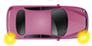
\includegraphics[width=\linewidth]{images/indicating_a}
		\label{fig:indicatinga}
\end{subfigure}
\begin{subfigure}{0.11\linewidth}
	\centering
	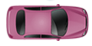
\includegraphics[width=\linewidth]{images/normal_a}
	\caption*{Aggressiv}
	\label{fig:normala}
\end{subfigure} 
\begin{subfigure}{0.1\linewidth}
		 \centering
		 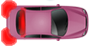
\includegraphics[width=\linewidth]{images/breaking_a}
		 \label{fig:breakinga}
\end{subfigure} 
\begin{subfigure}{0.1\linewidth}
		\centering
		
\includegraphics[width=\linewidth]{images/indicating_n}
		\label{fig:indicatingn}
\end{subfigure} 
\begin{subfigure}{0.11\linewidth}
	\centering
	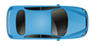
\includegraphics[width=\linewidth]{images/normal_n}
	\caption*{Neutral}
	\label{fig:normaln}
\end{subfigure} 
\begin{subfigure}{0.1\linewidth}
	\centering
	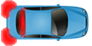
\includegraphics[width=\linewidth]{images/breaking_n}
	\label{fig:breakingn}
\end{subfigure} 
\begin{subfigure}{0.1\linewidth}
\centering
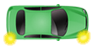
\includegraphics[width=\linewidth]{images/indicating_p}
\label{fig:indicatingp}
\end{subfigure}  
\begin{subfigure}{0.11\linewidth}
			\centering
			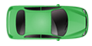
\includegraphics[width=\linewidth]{images/normal_p}
			\caption*{Passiv}
			\label{fig:normalp}
\end{subfigure} 
\begin{subfigure}{0.1\linewidth}
	\centering
	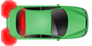
\includegraphics[width=\linewidth]{images/breaking_p}
	\label{fig:breakingp}
\end{subfigure}
\caption{Fahrzeugtypen: Aggressiv, Neutral, Passiv}
\label{fig:fahrzeug}
\end{figure}

\section{Spawner}
\textbf{Schwierigkeit:} Wie schafft man es einen realistischen Verkehrsfluss zu erzeugen, um den Eingangsverkehr in das Simulationsgebiet zu Simulieren.
%Wie schafft man es Fahrzeuge zu erzeugen, die mit einem realistischen Verkehrsverhalten an das Stauende fahren.
\begin{addmargin}[25pt]{0pt}
	\item \textbf{Lösungsansatz:} Da die Simulation lediglich ein beschränktes Gebiet betrachtet, ist es notwendig, dass in das Gebiet hineinfließende Verkehrsverhalten möglichst realistisch darzustellen. Hierbei beschr\"ankt sich das Modell auf folgende Aspekte: 
\begin{itemize}
	\item Der Sicherheitsabstand wird eingehalten.
	\item Fahrzeuge werden mit ähnlicher Geschwindigkeit erzeugt.
	\item Fahrzeuge fahren links schneller, aufgrund des rechtsseitigen Überholverbots.
	\item Auf der rechten Fahrspur gibt es eine höhere Verkehrsdichte.
\end{itemize}
Um ein neues Fahrzeug in die Simulationsumgebung einzuzufügen, wird eine normal verteilte Zufallszahl gewählt, welche den Zeitpunkt für die Erzeugung eines Autos beschreibt. Erwartungswert und Standardabweichung verhalten sich umgekehrt proportional zur gewünschten Verkehrsdichte. Ist dieser Zeitpunkt erreicht, wird anhand der voraus fahrenden Autos der vorhandene Platz berechnet. Damit ein Auto erzeugt werden kann, muss der vorhandene Platz mindestens den Sicherheitsabstand betragen. Zusätzlich wird die Geschwindigkeitsbeschränkung für das erzeugte Auto berechnet. Diese Geschwindigkeitsbeschränkung ist so definiert, dass das Auto noch genug Zeit zum Bremsen hat, um einen Unfall zu vermeiden. Eine ähnliche Geschwindigkeit wir dadurch gewährleistet, dass die Geschwindigkeit in Abhängigkeit der derzeitigen Verkehrsgeschwindigkeit berechnet wird, jedoch die Geschwindigkeitsbeschränkung nicht überschreiten darf. Zusätzlich müssen Fahrzeuge die auf der linken Spur erzeugt werden mindestens die Spurgeschwindigkeit der rechten Spur besitzen, um das rechtsseitige Überholen zu verhindern.
%TODO Fahrertypen??
\end{addmargin}

\section{Bedienung}
\textbf{Schwierigkeit:} Wie erhält man eine benutzerfreundliche Bedienungsoberfläche, bei der man möglichst viele Variablen verändern kann.
\begin{addmargin}[25pt]{0pt}
	\begin{figure}
		\begin{subfigure}{0.5\linewidth}
			\centering
			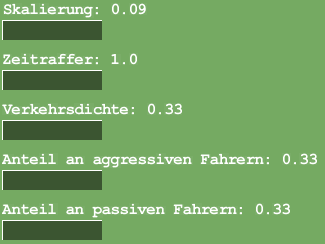
\includegraphics[width=\linewidth]{images/Eingabe}
			\caption*{Eingabefelder}
			\label{fig:eingabe}
		\end{subfigure}
		\begin{subfigure}{0.5\linewidth}
			\centering
			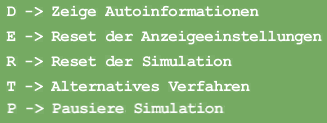
\includegraphics[width=\linewidth]{images/Bedienung}
			\caption*{Shortcuts}
			\label{fig:shortcuts}
		\end{subfigure}
	\caption{Bedienelemente}
	\label{fig:bedienung}
	\end{figure}
	
	\item \textbf{Lösungsansatz:} Die Steuerung über Eingabefelder (Abb.\ref{fig:bedienung}) hat sich als am benutzerfreundlichsten herausgestellt. Hier hat der Benutzer die Möglichkeit auf Skalierung, Zeitraffer, Verkehrsdichte, sowie den Anteil der Fahrertypen Einfluss zu nehmen. Um Fehler zu vermeiden, werden nur sinnvolle Eingaben berücksichtig.\\ 
Mithilfe der Skalierung kann man an die Verengung heranzoomen. Bei der Standardeinstellung von 0.09 wird der komplette Simulationsbereich betrachten.\\ 
Der Zeitraffer dient dazu Langzeitentwicklungen schneller darstellen zu können. Hierbei ist jedoch zu beachten, dass durch die Verwendung des Zeitraffers die Abtastrate sinkt. Dadurch kann es zu Genauigkeitsverlusten kommen. Bis zur fünffachen Geschwindigkeit sind die Ergebnisse noch relativ genau, bei einer schnelleren Betrachtung dient das Ergebnis lediglich als grobe Annäherung.\\
Durch die Verkehrsdichte kann man die Erzeugungswahrscheinlichkeit von Fahrzeugen verändern. Die Verkehrsdichte hat massgeblichen Einfluss auf die Effektivität des Reißverschlussverfahrens. Diesen Einfluss kann der Benutzer anhand der ausgegebenen Durchschnittsgeschwindigkeit, der Eingangsverkehrsdichte, sowie der Ausgangsverkehrsdichte ablesen.\\
Zu guter letzt kann der Benutzer noch den Anteil der Fahrertypen variieren. Standardmäßig gibt es 33\% aggressive (rosa), 33\% passive (grün) und 33\% neutrale Fahrer (blau). Die Anteile addieren sich immer zu 100\% auf, wobei die aggressiven und passiven Anteile durch Eingabefelder veränderbar sind und der neutrale Fahrer die restlichen Anteile bekommt.\\\\
	Zusätzlich wurden mehrere Shortcuts (Abb. \ref{fig:bedienung}) implementiert:
	\begin{itemize}
		\item \textbf{Verfahren wechseln}\\
		Mithilfe von "'T"' lässt sich das Reißverschlussverfahren wechseln. Hierbei werden zusätzlich alle Daten wieder zurückgesetzt.
		\item \textbf{Fahrzeugdaten anzeigen}\\
		Solle der Benutzer zusätzliche Informationen zu den jeweiligen Autos bekommen wollen, kann er durch Betätigung des "'D"' auf der Tastertur sich zu jedem Auto dessen ID, die derzeitige Geschwindigkeit, sowie die Beschleunigung anzeigen lassen. Diese Funktion wurde zum Debuggen erstellt, wodurch kein großer Wert auf die Lesbarkeit gelegt wurde und somit sich die Datenausgaben überlagern können.
		\item \textbf{Reset}\\
		Mithilfe von "'R"' kann man die Simulation reseten. Dabei werden alle Fahrzeuge entfernt.\\
		Wird "'E"' gedrückt werden alle getroffenen Einstellungen wieder auf die Standardeinstellung gesetzt.
		\item \textbf{Pause}\\
		"'P"' pausiert und setzt die Simulation fort.
	\end{itemize}
\end{addmargin}

\section{Fahrer}
\textbf{Schwierigkeit:} Es gibt in der Realität viele unterschiedliche Fahrertype. Jeder Fahrer hat einen individuellen Fahrstyle. Diese lassen sich häufig in Kategorien wie zum Beispiel aggressive oder passive Fahrer einordnen. Ganz ohne die Unterscheidung von Fahrertypen wäre die Simulation nicht Realitätsgetreu.
\begin{addmargin}[25pt]{0pt}
	\item \textbf{Lösungsansatz:} Die Programmierung von sehr vielen Fahrertypen ist zeitaufwendig und alle psychologischen Aspekte sind nicht darstellbar. Es wurden drei Fahrertypen implementiert: Der Aggressiven (rosa), der Neutralen (blau) und der Passiven (grün). Diese drei Fahrertypen unterscheiden sich darin, wie großen Sicherheitsabstand sie einhalten, mit welcher Geschwindigkeit sie erzeugt werden, wie stark der Fahrer abbremst sobald das vorausfahrende Fahrzeug bremst und wie sie sich beim Einsortieren verhalten. So hat der aggressive Fahrer eine deutlich höhere Wahrscheinlichkeit, dass er mit einer erhöhten Geschwindigkeit erzeugt wird, als der passive oder neutrale Fahrer. Zudem nutzt der aggressive Fahrer jede noch so kleine Lücke die sich bei der Verengung ergibt. Der Passive hingegen lässt einen deutlich größerenen Sicherheitsabstand zum vorausfahrenden Fahrzeug und hat einen höheren "Panikfaktor", welcher bewirkt, dass er sobald vorne gebremst wird, auch stark abbremst.\\
Um die Simulation realitätsgetreuer zu machen besitzt jeder Fahrer eine Reaktionszeit von 250\,ms. Dadurch bremsen nicht alle Fahrzeuge gleichzeitig sondern erst wenn der Vordermann auch bremst.\\
\end{addmargin}
\chapter{Interessante Recherche}
Während unser Recherche sind wir auf mehrere Studien bezüglich der Kooperationsbereitschaft gestoßen. Das Saulendiagramm (Abb. \ref{fig:kooperation}) gibt die Druchsschnittsgeschwindigkeit in Abhängigkeit der Eingangsverkehrsstärke, sowie des Kooperationsanteils an. Auffallend ist, dass abhängig von der Verkehrsdichte unterschiedliche Kooperationsanteile einen besseren Verkehrsfluss bieten. Bei einer Eingangsverkehrsstärke von bis zu 15\,$\frac{\text{Fahrzeugen}}{\text{min}}/\text{Spur}$ hat der Kooperationanteil noch keinen großen Einfluss auf den Verkehrsfluss. Unabhängig von ihrem Fahrverhalten passieren die Fahrzeuge die Engstelle mit ca. 115\,$\frac{\text{km}}{\text{h}}$ bei einem Eingangsverkehr von 10\,$\frac{\text{Fahrzeugen}}{\text{min}}/\text{Spur}$ beziehungsweise ca. 105\,$\frac{\text{km}}{\text{h}}$ bei 15\,$\frac{\text{Fahrzeugen}}{\text{min}}/\text{Spur}$.
Bei 20\,$\frac{\text{Fahrzeugen}}{\text{min}}/\text{Spur}$ ist die Durchnittsgeschwindigkeit am besten, wenn sich genau 50\% der Autofahrer an das Reißverschlussverfahren nach StVO halten. Überraschend ist, dass der Verkehrsfluss besser ist, wenn sich nur 15\% der Verkehrsteilnehmer an die Vorschriften halten, als wenn sich 85\% dran halten. Dieses Phanomen ändert sich jedoch ab einer Eingangsverkehrsstärke von 25\,$\frac{\text{Fahrzeugen}}{\text{min}}/\text{Spur}$, bei welcher die bestmögliche Durchschnittsgeschwindigkeit von 50\,$\frac{\text{km}}{\text{h}}$ bei hoher Kooperaionsbereitschaft existiert.\\
\begin{figure}
	\centering
	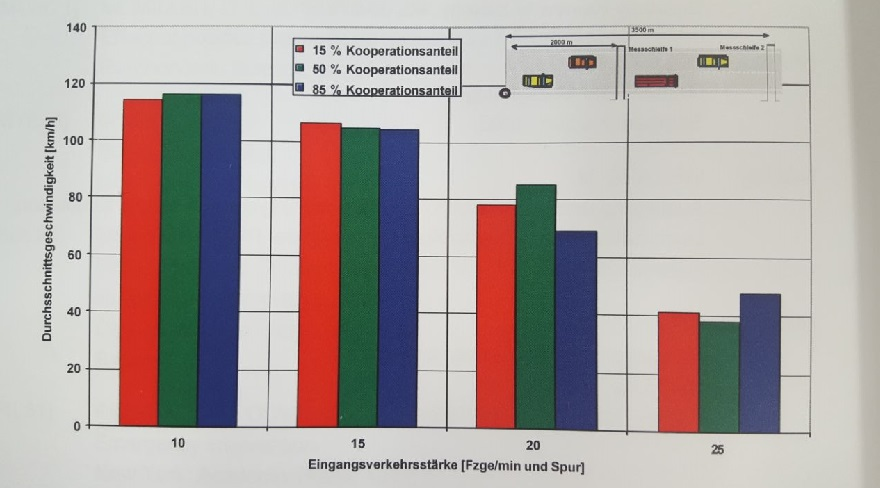
\includegraphics[width=0.6\linewidth]{images/Kooperation}
	\caption{Durchschnittsgeschwindigkeit im Szenario "'Autobahn bei hoher Dynamik und Dichte"'}
	\label{fig:kooperation}
\end{figure}
Diese Studie unterstreicht die Wichtigkeit, Fahrertypen zu implementieren, die einen unterschiedlichen Kooperationsanteil besitzen um ein realistisches Ergebnis zu erhalten.
\chapter{Weiterführend}
Weiterführende Verbesserungen der Simulation könnten in folgenden Bereichen implementiert werden:
\begin{itemize}
	\item \textbf{Debuggen:}
	\begin{figure}
		\centering
		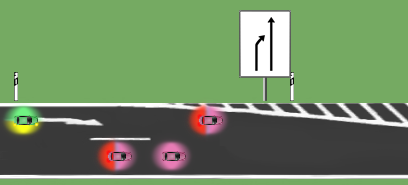
\includegraphics[width=0.7\linewidth]{images/BUG}
		\caption{Rosa Auto ist zuweit gefahren}
		\label{fig:bug}
	\end{figure}

Die Simulation besitzt noch mehrere Bugs. Wenn das Verkehrsvorkommen zu hoch ist, fahren manche Autos einfach über das Hindernis hinweg oder bleiben davor stehen, erkennen aber keine Lücke mehr. Das Problem dabei ist, dass die Fahrzeuge auf der rechten Seite das Fahrzeug noch erkennen und bremsen um dieses reinzulassen. Dadurch kommt es zu unnötigem und realtitätsfernem Rückstau.
Auch der Fahrbahnwechsel ist noch nicht perfekt implementiert. Das Fahrzeug erkennt, wenn es auf der stärker befahrerenen Spur ist und wechselt auf die andere Fahrbahn, jedoch ist dieser Wechsel nicht immer sinnvoll.
\item \textbf{Ein weiteres Verfahren:}\\
Es wäre interessant ein Verfahren zu entwickeln was davon aus geht, dass nur autonome Fahrzeuge beteiligt sind. So könnten aufgrund der Kommunikation zwischen den Fahrzeugen statt Lücken suchen zu lassen, Lücken  gebildet werden, welche dann dem jeweiligen Fahrzeug zugewiesen werden. Diese Verfahren dürfte das Effektivste sein, jedoch frühestens in 20 Jahren von Bedeutung.

\item \textbf{Eine dritte Spur:}\\
Die Effektivität eines Einfädelungsverfahrens ist abhängig von der Anzahl der Spuren. Wenn die Fahrbahn von drei auf zwei Fahrbahnen verengt wird, verhält sich der Verkehr anders, als wenn aus zwei eine Fahrbahn wird. Es gibt viel mehr Platz und es gibt zwei Spuren welche die Engstelle passieren, wodurch der Verkehrsfluss wahrscheinlich besser ist.

\item \textbf{Weitere Fahrzeugarten:}\\
Die Simulation enthält nur eine Art von Fahrzeug. Diese hat eine einheitliche Länge von 4,5\,m und die Breite wird nicht betrachtet. Es kommt jedoch vor, dass in Baustellen die linke Fahrspur nur für Fahrzeuge bis 2,1\,m freigegeben ist.
Zudem wäre es interessant den Einfluss von LKWs oder Wohnwagen auf das Reißverschlussverfahren zu untersuchen.

\item \textbf{Mehr Fahrertypen:}\\
Um eine aussagekräftige Simulation zu erhalten, reicht es aus alle Fahrer in die Kategorien aggressiv, neutral, und passiv, zu unterteilen. In der Realität hat jedoch jeder Fahrer seinen individuellen Fahrstil. Deshalb wäre es interessant, noch mehr Fahrertypen zu ergänzen und detaillierter in ihren Eigenschaften zu beschreiben.

\item \textbf{Verhalten bei Unfällen:}\\
In der derzeitigen Version werden Unfälle zur Kenntnis genommen, aber nicht beachtet. Wenn Autos kollidieren wird lediglich eine Statusmeldung angezeigt, die Geschwindigkeit wir auf 0\,$ \frac{\text{km}}{\text{h}} $, jedoch fahren die Fahrzeuge danach ganz normal weiter.

\item \textbf{Unterschiedliche Gegebenheiten:}\\
Es macht einen Unterschied, ob ein Reißverschlussverfahren auf der Autobahn oder in der Stadt eingesetzt wird, da die Anfangsgeschwindigkeiten unterschiedlich sind und in der Stadt auch Ampeln zu berücksichtigen sind.\\
Zudem macht es einen Unterschied, ob die Verengung Aufgrund einer Baustelle oder eines Unfalls entsteht. Im Falle eines Unfalls könnte man zusätzlich eine Rettungsgasse simulieren.
\end{itemize}
\chapter{Fazit}
Beide Verfahren haben ihre Vor- und Nachteile. Nach betrachten unterschiedlicher Verkehrsvorkommen sind wir zu dem Fazit gelangt, dass das Reißverschlussverfahren nach StVO, zurzeit das bessere Verfahren ist.
Das liegt daran, dass das alternativ getestete Reißverschlussverfahren bei hoher Verkehrsdichte seine Effektivität verliert. Da nicht jede Lücke optimal genutzt wird, kommt es zu einem gravierent längeren Rückstau, welcher gegebenenfalls zusätzlich Zufahrtsstraßen verstopft. Bei niedrigem Verkehrsvorkommen ist es jedoch, wie erwartet die bessere Methode. Da jedoch auf Autobahnen eher mit einer hohen Verkehrsdichte zu rechnen ist, haben diese Ergebnisse eine besonders hohe Gewichtung. Zudem ist das alternativ getestete Verfahren, wegen der Benötigten frühzeitigen Ankündigung, nur bei Baustellen nutzbar, während das jetztige Reißverschlussverfahren auch bei Hindernissen wie Unfällen gut einsetzbar ist.\\
Sollte es in ferner Zukunft zur Einführung von autonom fahrenden Fahrzeugen kommen, welche miteinander kommunizieren können, wäre das alternative Verfahren das Geeignetere. Dies liegt daran, dass der Beginn des Reißverschlussverfahren nicht durch Verkehrsschilder eingeleitet wird, sondern durch Kommunikation zwischen den Fahrzeugen, wodurch der Beginn des Einfädelungsprozess der Verkehrsdichte angepasst werden kann.
%Literaturverzeichnis
%\bibliographystyle{plaindin}
\bibliography{literatur}
\bibliographystyle{plain}
%Appendix
\appendix
%\chapter{Anhang}
\section{UML Diagramme}
\subsection{Klassendiagramm}
\begin{figure}
	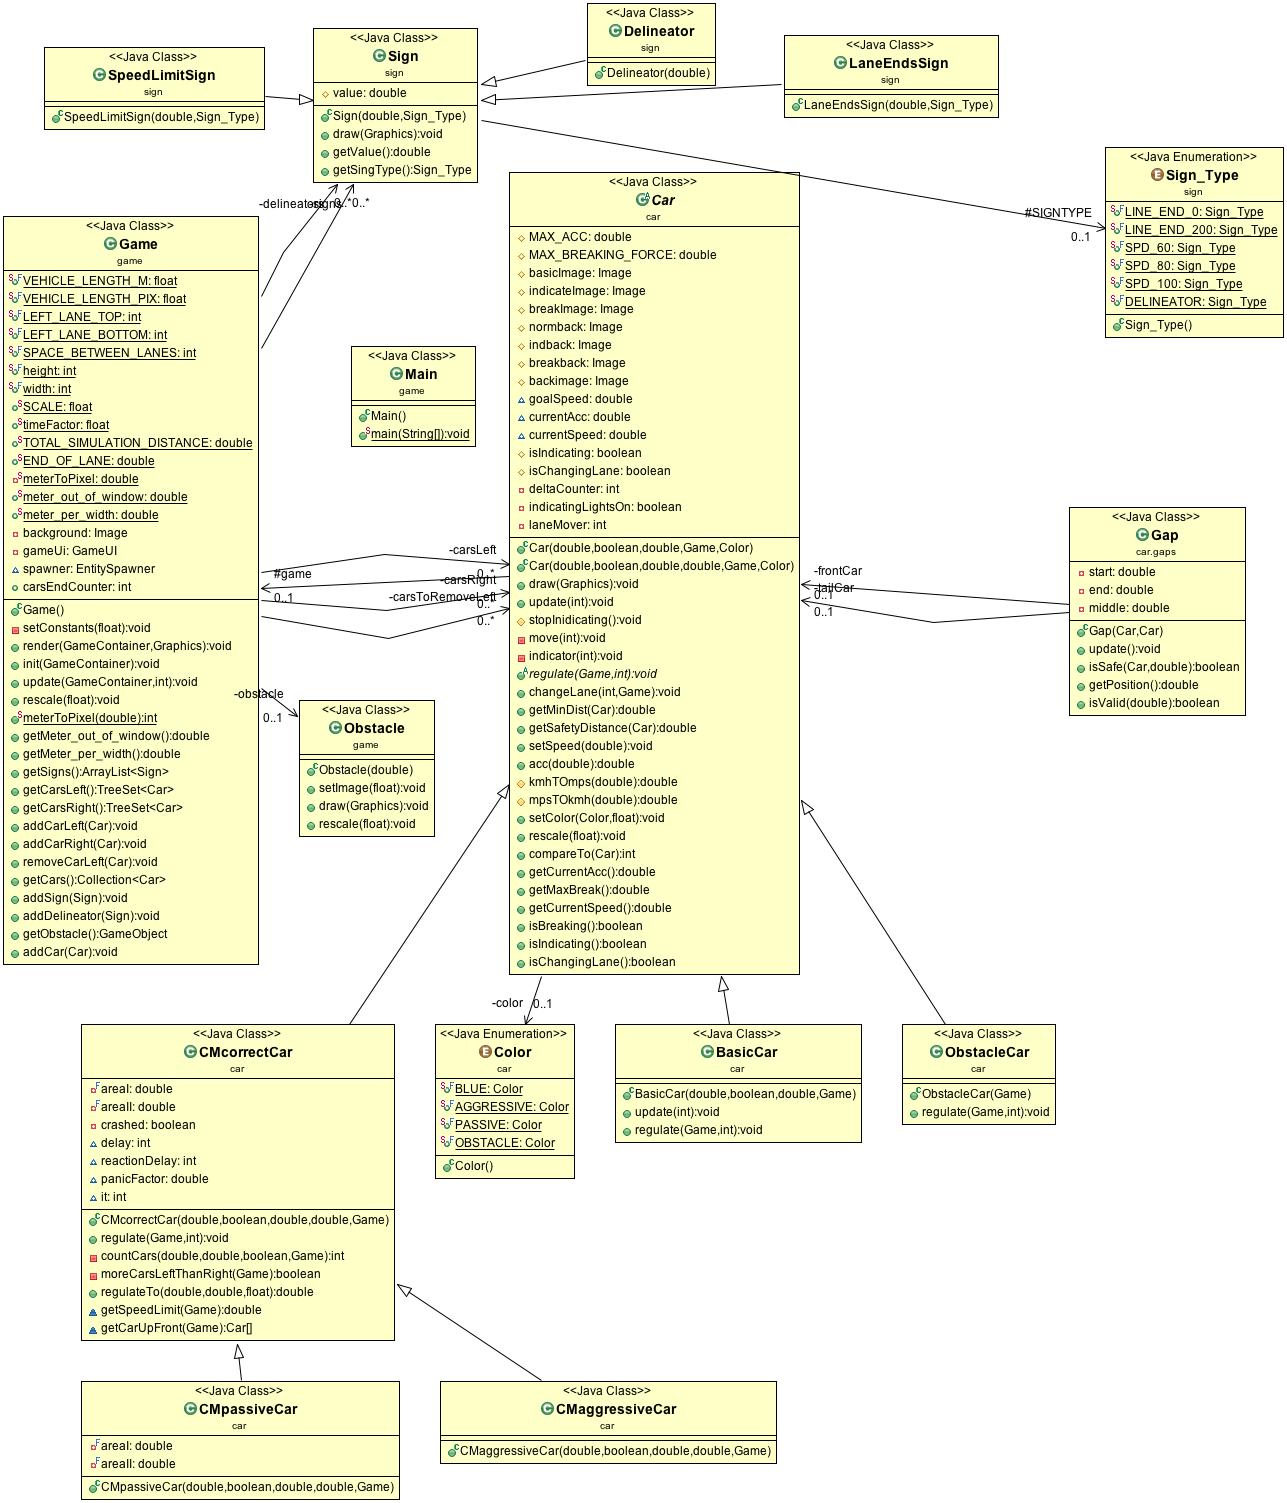
\includegraphics[width=\linewidth]{images/classuml.png}
	\caption{UML Klassendiagramm}
	\label{fig:umlclass}
	\end{figure}

\end{document}